\chapter{Design}%
\label{cha:design}

%In this chapter, you should present your solution in detail but at a conceptual level. This means that you explain the overall design including your motivation for this design but you do not provide details on the actual implementation of your design (e.g., in which programming language you wrote it, how the software is structured and so on). This means that you should also point out the aspects where you had different design options and in which points they differ. A good approach to write this chapter is to make yourself aware of the different aspects and design problems that need to be addressed in your design. To do so, you can then proceed repeatedly in three steps:
%\begin{enumerate}
 %  \item Explain a design problem that needs to addressed by the solution (e.g. to enable anonymous communication over the internet, participants need to be able to send messages to each other without revealing identifying to the corresponding receiver).
  % \item Discussion of design choices (e.g. Mix Networks, DC-Networks, etc.) with regards to the requirements from the previous chapter and identification of the most promising choices.
%\end{enumerate}
%After the second step, you start the next iteration by identifying design problems that arise when you want to use the most promising design choice. For example, if Mix networks turn out to be the most promising approach for your requirements, you then need to address the question how the mix network should be designed (e.g. how are mix nodes chosen by the users of the anonymization network? How do mix nodes process messages?). Once you identified the most promising solutions to that, you can then start the next iteration and so on until there are no more open design questions that you are aware of.
Zuerst wird die Notwendigkeit für eine Taxonomie erläutert. Dann erfolgt die Definition der Taxonomiekategorien. Danach wird festgelegt in welcher Form die Kontextinformationen in den einzelnen Kategorien vorliegen müssen und wie man Informationen aus unterschiedlichen Quellen in einer für sammelt. Zusätzlich wird noch darauf eingegangen welche Anforderungen ein IDS erfüllen sollte, welche davon im speziellen für diese Arbeit relevant sind und welche Schwächen des IDS mithilfe des vorgeschlagenen Designs und Kontextsensitivität gelöst werden. 

\section{Notwendigkeit einer Taxonomie}
%TODO “Based on the evaluation of context categorisation, it is evident that no single categorisation scheme can accommodate all the demands” ([Perera et al., 2014, p. 423]
Die Evaluation verschiedener Kategorisierungsschemata zeigt das keine Kategorisierung allen Ansprüchen gerecht werden kann \cite{perera_context_2014}.
\section{ Erstellung einer Kontexttaxonomie }
Im folgenden möchte ich meinen Versuch einer Kombination der bereits vorgeschlagenen Kategorisierungsschemata erläutern. Dazu lege ich zuerst die Definition der einzelnen Kategorien im Bezug auf kontextsensitive Zugriffskontrolle fest. Die Kategorien müssen dafür, abhängig davon mit welchem Fokus sie der jeweilige Autor konstruiert hat, mehr oder weniger stark angepasst werden.
\subsection{Konzeptionell}
Einordnung anhand der Bedeutung des Kontextes und der begrifflichen Beziehungen.
\subsubsection{Primär}
%“Any information retrieved without using existing context and without performing any kind of sensor data fusion operations (e.g. GPS sensor readings as location information).” 
Kontextinformationen die gesammelt werden können ohne bereits vorhandene Daten zu verwenden oder zu kombinieren \cite{abowd_towards_1999}. 
\subsubsection{Sekundär}
%"Any information that can be computed using primary context. The secondary context can be computed by using sensor data fusion operations or data retrieval operations such as web service calls (e.g. identify the distance between two sensors by applying sensor data fusion operations on two raw GPS sensor values). Further, retrieved context such as phone numbers, addresses, email addresses, birthdays, list of friends from a contact information provider based on a personal identity as the primary context can also be identified as secondary context.” 
Kontext der durch das verarbeiten von primärem Kontext erschlossen werden kann. Dies kann durch die Kombination einzelner Datenpunkte einer oder mehrerer Kategorien oder durch Abfragen weiterer Informationen mithilfe der primären Informationen geschehen \cite{abowd_towards_1999}.
\subsection{Betrieblich}
Wie schon in der Analyse bereits vorgeschlagener Kategorien bedeutet die betriebliche Kategorisierung: ``Einordnung anhand dessen wie der Kontext akquiriert, modelliert und behandelt wird ''.
\paragraph{Zeit}
Zu welcher Zeit ein Zugriffsanfrage erfolgt.
\paragraph{Ort}
Von welchem Ort eine Zugriffsanfrage stammt.
\paragraph{Identität}
Wer Zugriff auf eine Ressource erfragt.
\paragraph{Aktivität}
Was in einer Situation passiert bzw. welche Aktion eine Entität ausführt.
\paragraph{Grund}
Warum etwas getan wird.
\begin{figure}[h!]
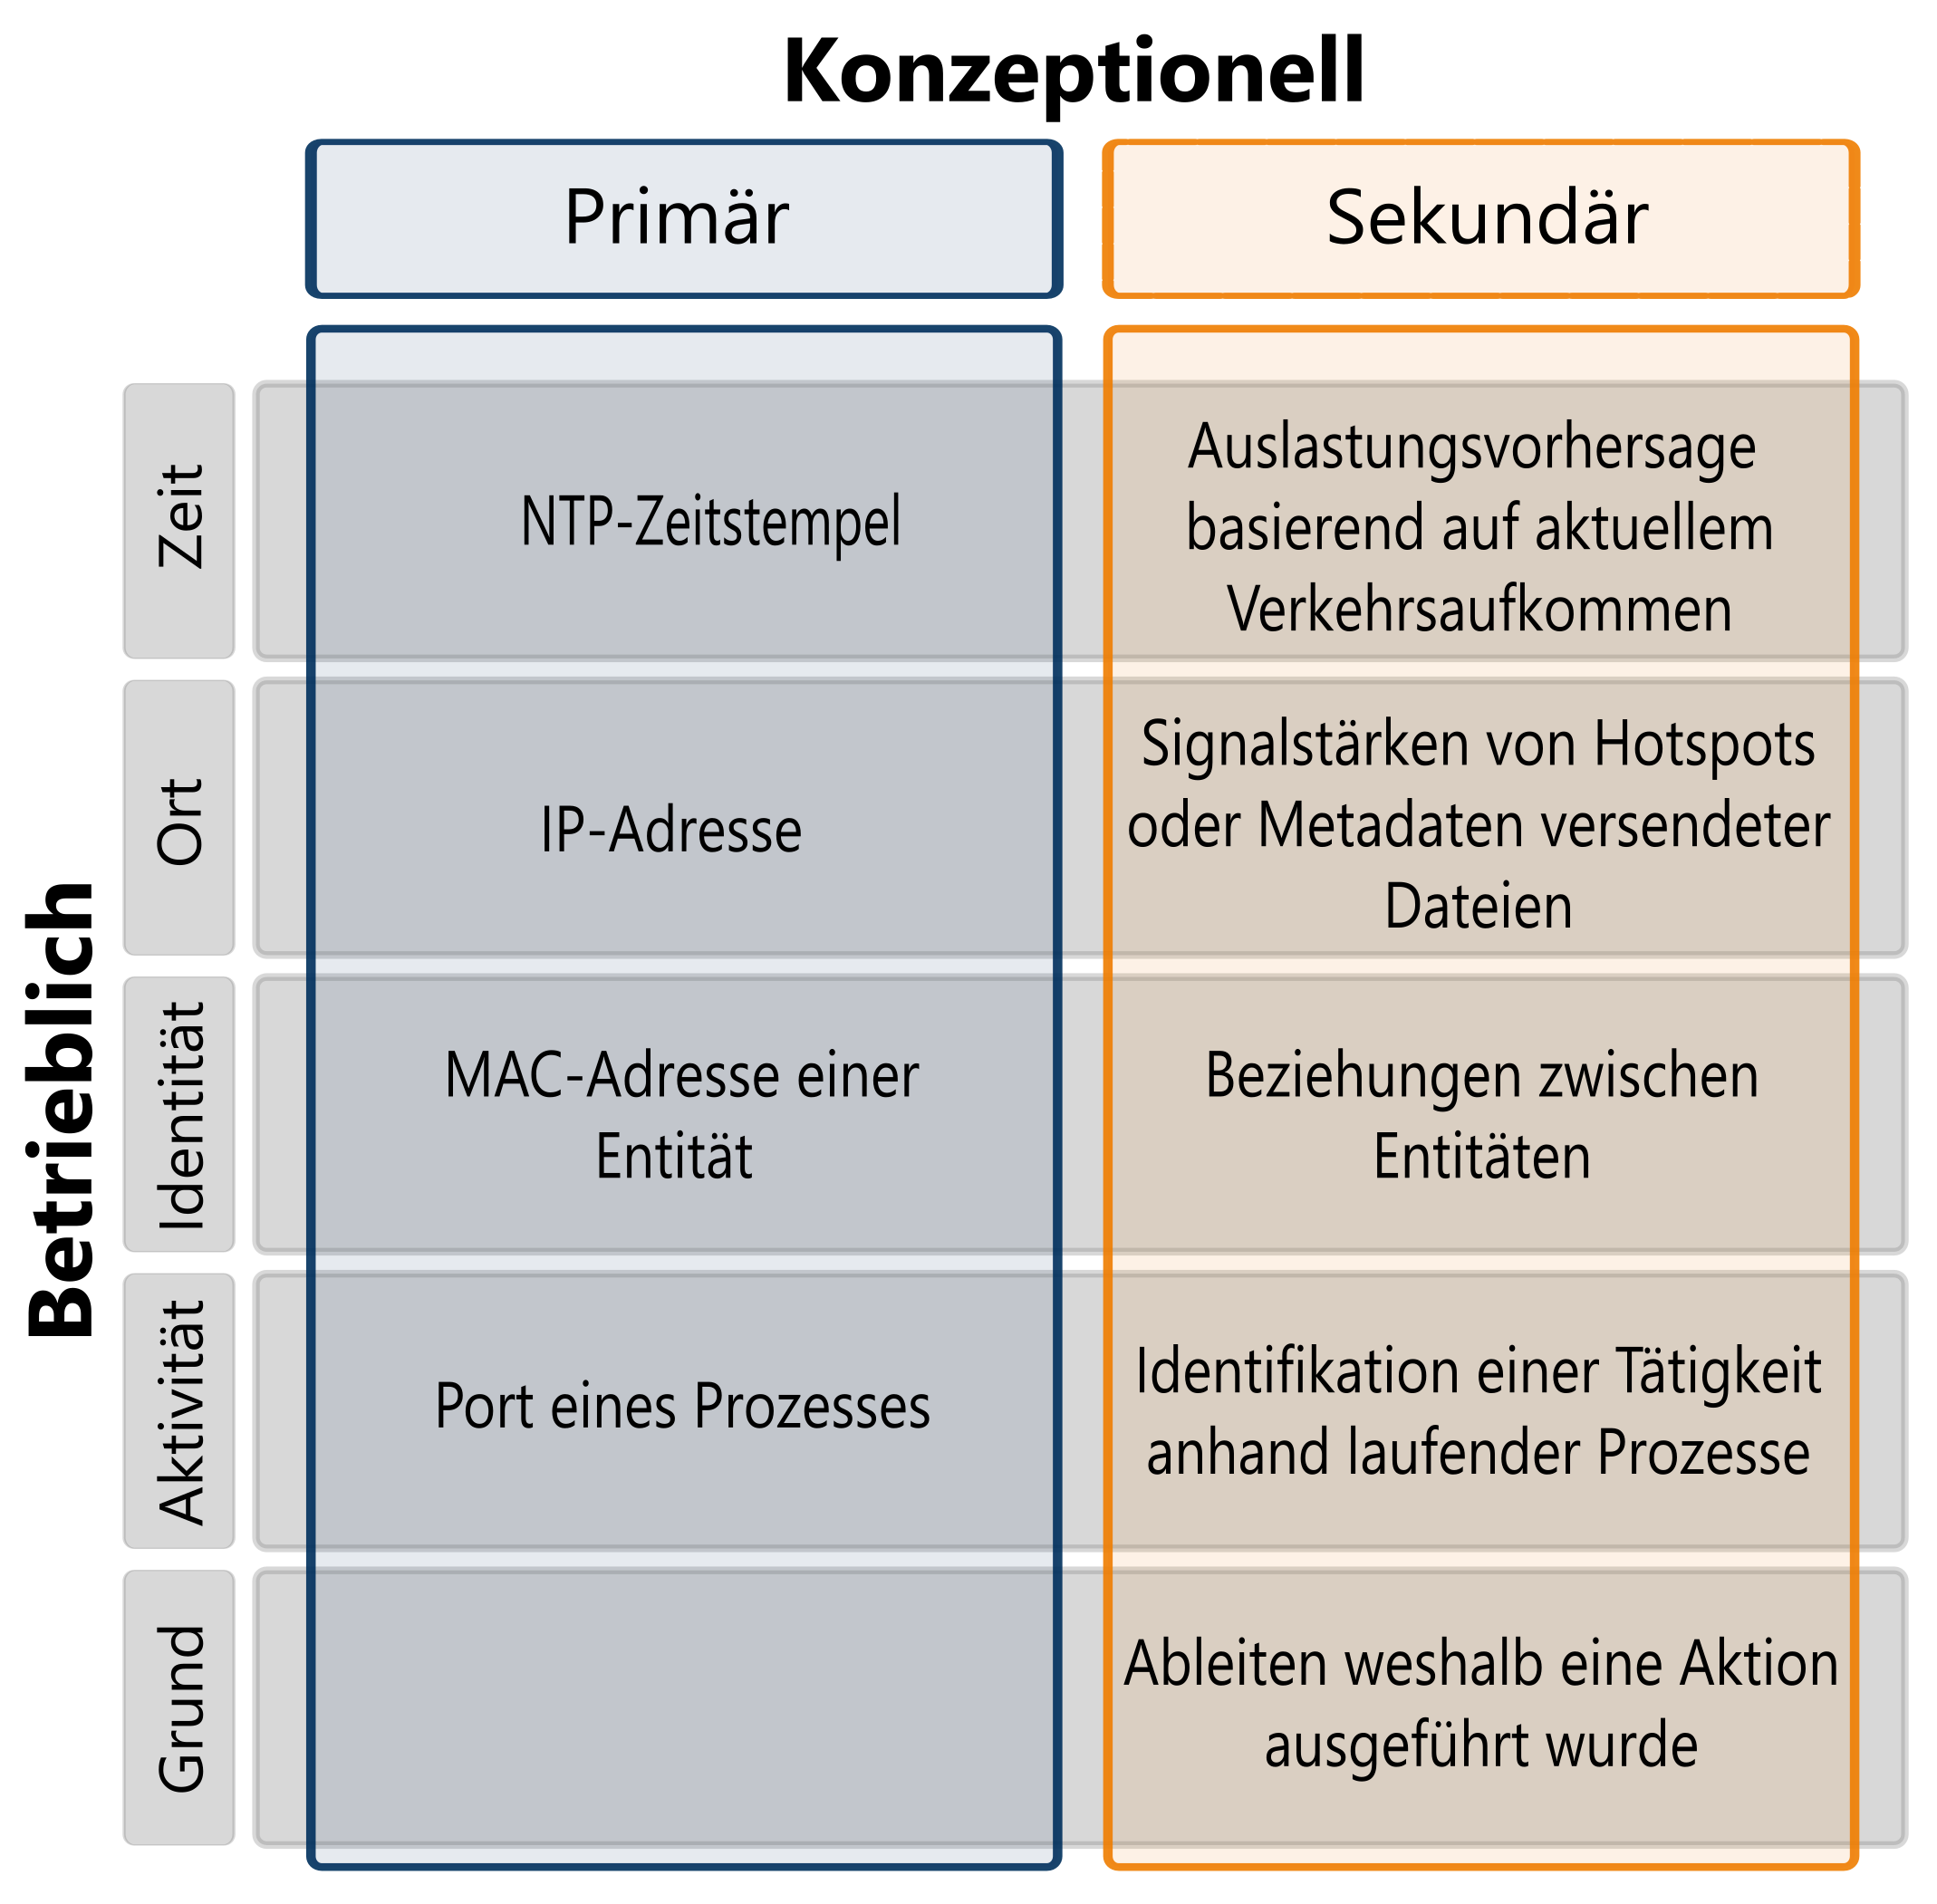
\includegraphics[width=15cm,height=15.2569cm]{graphic_1}
\caption{•}
\end{figure}
%--------------------------
\subsection{Historie}
Die Historie einer Entität wird in dieser Taxonomie zweigeteilt. Sie besteht aus:
\begin{enumerate}
\item{Einem aktiven Teil also ihrem Verhalten, beispielsweise früheren Verbindungen bzw. Verbindungsanfragen}
\item{Einem passiven Teil also dem Zustand der für sie charakteristischen Attribute, beispielsweise einem Nutzernamen oder die Versionsnummer eines bestimmten Programms}
\end{enumerate}
Die Existenz einer Historie trifft die implizite Annahme das eine Entität eindeutig und über einen längeren Zeitraum im Netzwerkverkehr identifizierbar ist.
\subsubsection{Dynamik}
Wie 
 %TODO im Kapitel Hintergrund%
 beschrieben können sich die Werte, aus denen sich die Historie einer Entität zusammensetzt, je nach dem welchem Teil sie zugeordnet werden, verschieden oft ändern.
Statische Messgrößen ändern dabei ihre Werte nie oder nur sehr selten. Dynamische Messgrößen hingegen sehr oft. In diesem Fall wird eine Unterteilung in jährlich, monatlich, wöchentlich, täglich, stündlich, minütlich und sekündlich vorgenommen.
\subsubsection{Raten}
Die Historie ist weiterhin in 3 verschiedene Bereiche unterteilt. Abhängig davon wo die Änderung auftritt und ob das IDS oder eine Entität die Aktualisierung des Wertes auslöst.
\paragraph{Änderungsrate} 
Gibt an wie oft eine Entität eine Werteänderungen mitteilt.
\paragraph{Abtastrate}
Wie oft Werte einer Entität vom IDS abgefragt bzw aktualisiert werden.
\paragraph{Abfragerate}
Wie oft Werte im Netzwerk von einer Entität, die nicht das IDS ist, abgefragt werden.
\begin{figure}[h!]
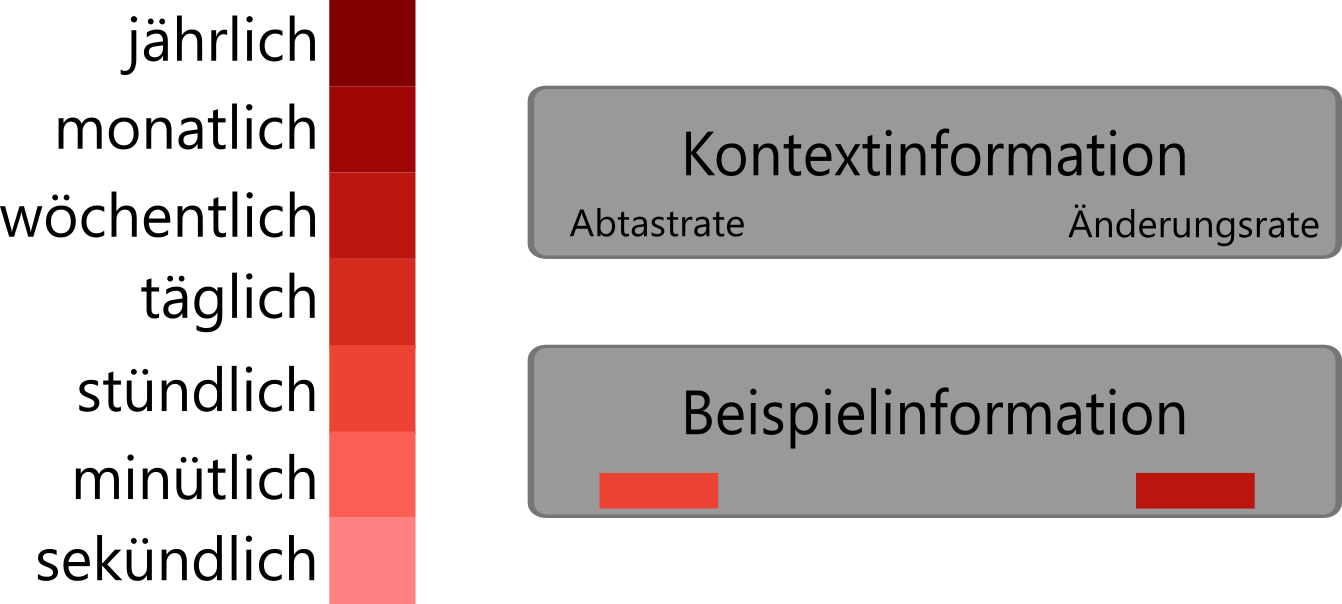
\includegraphics{history}
\caption{•}
\end{figure}
\pagebreak
%--------------------------

\subsection{Netzwerk}
Ein Netzwerk besteht im allgemeinen aus:
\begin{enumerate}
\item{Entitäten die daran teilnehmen}
\item{Kommunikation zwischen den Entitäten}
\item{Annahmen bzw. Normen bezüglich:}
\begin{enumerate}
	\item{des Verhaltens und der Eigenschaften der Entitäten}
	\item{der Form und dem Inhalt der Kommunikation}
\end{enumerate}
\end{enumerate}
In Rahmen der Zugriffskontrolle erfolgt Kommunikation im Netzwerk über spezifische Protokolle zwischen verschiedenen Entitäten die durch bestimmte Attribute charakterisiert werden. Die Normen werden dabei initial festgelegt und im Verlauf der Lebenszeit des Netzwerkes angepasst.  
\subsubsection{Protokolle}
Kategorisierung anhand des verwendeten Kommunikationsprotokolls. Orientiert sich am ISO/OSI-Referenzmodell \cite{day1983osi}. Die Zuordnung zu einer bestimmten Schicht und damit Kategorie erfolgt anhand der für die einzelnen Schichten üblichen Protokolle. Das ermöglicht die Identifikation von Entitäten anhand der von ihnen genutzten Protokolle. So kann beispielsweise ein Switch oder Router von einem Nutzer oder einer Anwendung unterschieden werden.
\paragraph{Anwendung}
Beinhaltet allen Netzwerkverkehr der sich der Sitzungsschicht, Darstellungsschicht oder Anwendungsschicht zuordnen lässt 
\paragraph{Transport}
Pakete die sich der Transportschicht zuordnen lassen.
\paragraph{Vermittlung}
Netzwerkverkehr der zur Vermittlungsschicht gehört.
\subsubsection{Entitäten}
Kategorisierung von Kontextinformationen abhängig davon welche Art von Entität sie betreffen.
Diese Unterscheidung setzt genauso wie die Historie eindeutig identifizierbare Entitäten voraus.
\paragraph{Gerät}
Informationen die sich auf ein spezifisches Gerät beziehen
\begin{enumerate}
\item{Ein Gerät ist beispielsweise einen Router oder das Endgerät eines Nutzers. }
\item{Informationen können beispielsweise die Liste an installierter Software, die Menge laufender Prozesse oder die Auslastung der Hardwarekomponenten sein.}
\end{enumerate}
\paragraph{Nutzer}
Informationen die sich auf einen Nutzer beziehen.
\begin{enumerate}
\item{Ein Nutzer im Sinne eines Computersystems und keine physische Person. So kann eine physische Person durchaus mehrere verschiedene logische Nutzerkonten haben. }
\item{Informationen können zum Beispiel die Zugriffsrechte eines Nutzers sein.}
\end{enumerate}
\paragraph{Anwendung}
Informationen die sich auf eine Anwendung beziehen.
\begin{enumerate}
\item{Anwendung umfasst jegliche Softwareprozesse die für sich oder in Kombination einen bestimmten Zweck erfüllen.}
\item{Eine Anwendung erzeugt für sie charakteristischen Netzwerkverkehr, versendet oder empfängt also bestimmte Informationen.}
\end{enumerate}
\subsubsection{Normen}
Einordnung der Kontextinformationen abhängig davon ob sie der für den Anwendungsfall definierten Normen entsprechen.
\paragraph{Erwartet}
Form der Kommunikation mit verschiedenen Protokollen oder Verhalten von Entitäten passend zu den im Netzwerk vorherrschenden Bedingungen.
\paragraph{Ungewöhnlich}
Form der Kommunikation mit verschiedenen Protokollen oder Verhalten von Entitäten die in Kombination mit den im Netzwerk vorherrschenden Bedingungen entweder auffällig oder irrational sind.
\newpage
\begin{figure}[h!]
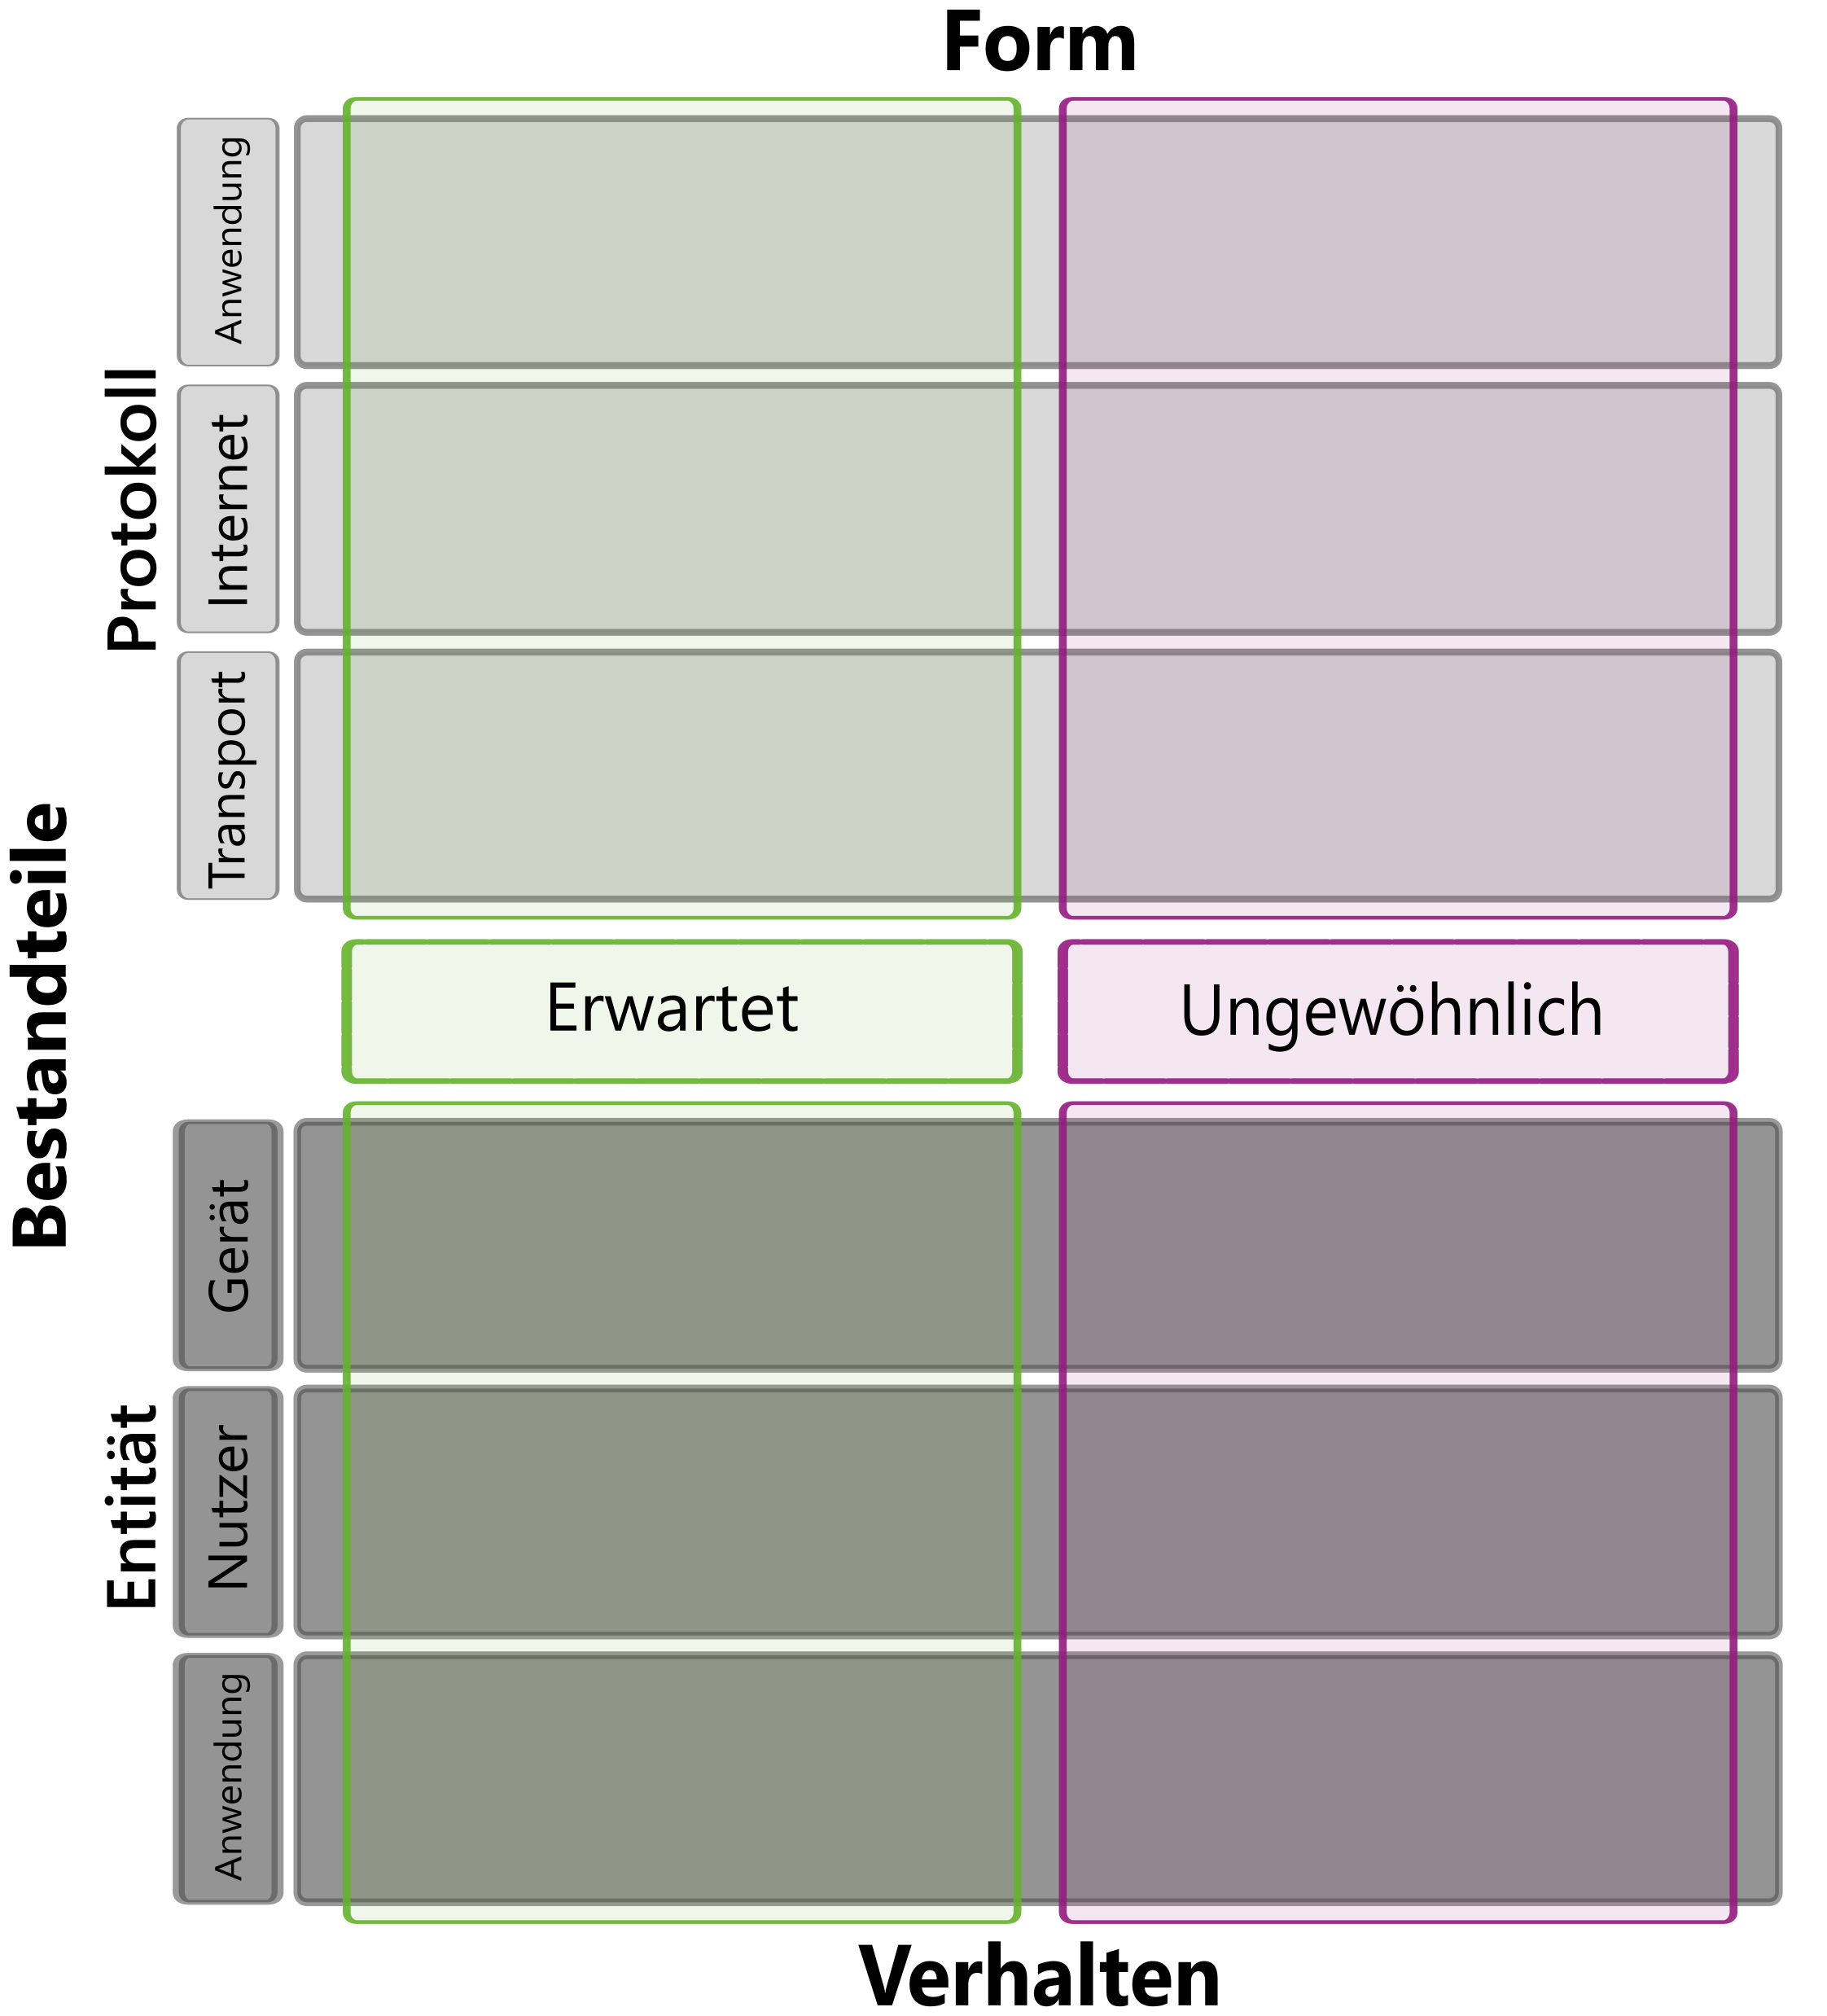
\includegraphics[width=15cm,height=16.97cm]{graphic_2}
\caption{Kategorisierung von Kontextinformationen als Bestandteile eines Netzwerkes}
\end{figure}
\newpage

\section{Form des Kontextes}
Nachdem die einzelnen Kategorien definiert wurden muss festgelegt werden in welcher Form die Kontextinformationen vorliegen sollen bzw. gebracht werden müssen. Dies ist hauptsächlich davon abhängig wie die Informationen in das IDS eingelesen werden.


%TODO work in Progress

\subsection{Historie}
Die Historie einer Entität muss genug Informationen enthalten um damit neue Entscheidungen in der Gegenwart oder Zukunft zu treffen und sie eindeutig zu identifizieren. Die Identifikation erfolgt anhand der Headerinformationen der einzelnen  Kommunikationsschichten. In der Historie gespeichert werden in entweder die gesamte Payload eines Pakets oder zumindest ein ausreichend aussagekräftiges Subset. Die Regelmäßigkeit mit der die Historie aktualisiert bzw. erweitert wird ist vom jeweiligen Gegebenheiten und Ansprüchen abhängig.
\begin{figure}[h!]
\begin{tabularx}{1\textwidth} { 
  | >{\raggedright\arraybackslash}X 
  | >{\raggedright\arraybackslash}X 
  | }
 \hline
 Identifikationsmerkmale der Anfrage & Zugriffsentscheidung \\
 \hline
 MAC-Adresse & MAC-Adresse des Ziels  \\\hline
 IP-Adresse &  IP-Adresse des Ziels, gesetzte Flags, TTL, Protokoll \\\hline
 Port & Port des Ziels, protokollspezifische Informationen\\
 		& 			\\
\hline
\end{tabularx}

\end{figure}

%Scr-IP/Port + Dest-IP/Port
%Zeitpunkt
%Protokoll
%Paketlänge
%Verbindung möglich
%Verbindung zugelassen
\section{Kontextgewinnung}
%Wo genau bekommt man Kontextinformationen her 
.
Dabei sollte man bedenken an welcher Stelle und wie oft man Informationen abruft oder automatisch aktualisiert. \cite{perera_context_2014}

Es folgt eine Übersicht einiger Beispiele für Möglichkeiten Kontextinformationen zu gewinnen. 
%TODO  A Context Aware Network-IDS
- osquery
- network (open ports) | Nessus
- devices in network | Configuration Management Database (CMDB), nmap   
- cve reference - yes/no
- protocol header

